\graphicspath{ {../body/handover_figures/}}
\chapter{高速移动用户的无线网络基站切换算法}
\label{chap_iccs_handover_alogrithm}
本章针对在WiMAX网络中,高速移动用户基站切换算法问题。对于用户切换的流程进行分析,建立了一个WiMAX基站切换信令协议的交互概率模型。通过对此模型的分析,提出了一个用于在高速移动速度下保证切换成功的前向纠错方法。该方法在提供了一个方法通过增加额外的保护来保证切换过程的完成。通过仿真实验表明,所提出的方案可以通过计算在不同的移动速度下达到所需冗余比特数来达到认定的基站切换成功率。

\section{引言}
\label{section_iccs_handover_algorithm_introduction}
无线网络通信领域的高速数据服务总是需要宽带无线访问技术的支持。WiMAX ~(World Interoperrability for Microwave Access)是一项替代现在有线宽带访问技术如ADSL,提供最后一公里的无线网络接入技术。它提供一种方便快速的方法来建立无线城域网(WMN,wireless metropolitan area network)。这项技术可以对高速数据业务如宽带互联网访问,VoIP(Voice over Internet Protocol),IPTV等高速数据应用提供技术支持。WiMAX技术用来支持在基站与固定、移动或漫游用户终端之间的高速数据连接。固定WiMAX (IEEE 802.16-2004)的标准中定义了面向连接的媒体访问层(MAC)和基于正交频分复用(OFDM,orthogonal frequency division multiplexing)的物理层协议 \cite{IEEE:802_16D:2005}。而移动WiMAX(IEEE 802.16e-2005)的标准中还规定了对于移动用户所需的各种MAC层和物理层协议\cite{IEEE:802_16E:2006}。

%%%%%%%%%%%%%%%%%%%%%%%%%%%%%%%%%%%%%%%%%%%%%%%%%%%%%%%%%%%%%%%%%%%%%
\begin{figure}[htbp]
\begin{centering}
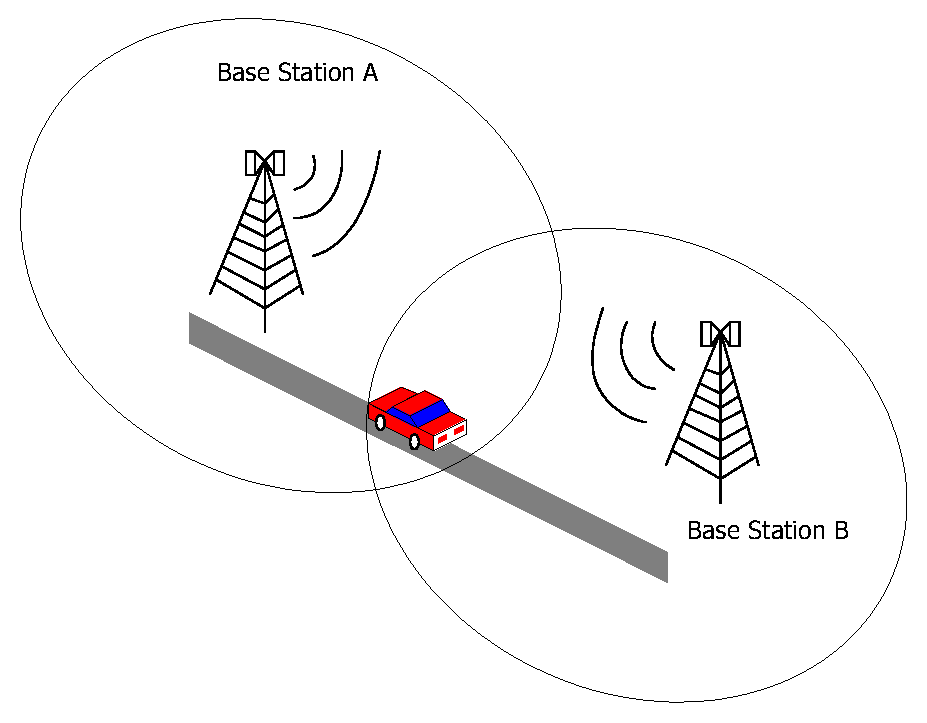
\includegraphics[width=9cm]{../figures/iccs_handover_bs}
%\caption{Simulation results of the probability of a handover success using the proposed adaptive FEC scheme.}
\caption{基站切换示意图}
\label{fig:chap_iccs_handover_bs}
\end{centering}
\end{figure}
%%%%%%%%%%%%%%%%%%%%%%%%%%%%%%%%%%%%%%%%%%%%%%%%%%%%%%%%%%%%%%%%%%%%%

在无线移动通信中,基站切换是一个非常重要的组成部分。它可以保证在用户在移动过程中(从一个地理位置到另一个地理位置,如图\ref{fig:chap_iccs_handover_bs}),用户的通信保持不被中断\cite{Pollini:1996:THD}\cite{Wright:ICMB2007}。基站切换可以是在同一网络中的小区切换(也被称为微移动性,Micro-mobility),也可以在不同的网络中的切换。譬如是无线局域网(WiFi)与移动通信网之间的切换。当前的移动WiMAX标准详细定义了在切换过程中所需的切换信令协议。这些协议用来在单点到多点(Point-to-multipoint,PMP)模式的通信中支持切换过程。通常,切换技术可以分成两种:软切换(Soft handover, SHO)和硬切换(Hard Handover,HHO)。在软切换过程中,移动台在切断与原有基站通信的之前,就已经完成和目标基站的切换信令,并建立了正常的通信连接。而在硬切换过程中,移动台先要完成断开与原有服务基站的连接,然后再与重新目标基站建立连接。显然,软切换的优点在于在切换的过程中,数据连接始终存在。但是同时的资源利用率较硬切换要低。硬切换过程中,数据连接会在一个段时间内是断开的。由此引入了一些延时,对于时间敏感的应用而言,也需要做专门地处理和优化来确保服务质量。通常对于时间敏感的应用,软切换也必须要进行一些优化的处理才能保证在移动WiMAX中QoS。

近些年来,对于软切换方面的研究,许多学者做了许多工作。他们中一部分人的工作的特点是集中在对于目标基站的选择上。通过对移动台的位置变化的预测、收集分析相邻基站的QoS信息或是对基站信号的分析来优化目标基站的选择\cite{Hsieh:INFOCOM2003}\cite{DooHwan:WPC2006}。另外一些人工作主要是集中在提高某些QoS的指标。在文献\cite{MinsikICACT2006}中,为了解决在切换过程中丢包率增加的问题,作者设计了一种交叉层的方法,在上层设备中如(网络层中的路由器)缓存切换移动台的数据。在文献\cite{JenHui:AUSWIRELESS:2007}中,Chen等学者为了减少在切换过程中的延时,提出了一种预协商的机制。这个机制利用预测移动台与基站间的距离,提前在目标基站中分配所需要的资源。在文献\cite{LingVTC2007}中,作者通过用IP层的链路来传送MAC层的信息来达到减少切换延时的目的。还有一些学者的研究集中在对切换中出现的CID分配冲突提出了更加合理的分配方案或是对移动台的数据进行分类处理,最终也可以提高QoS的水平\cite{Hu:TVT2004}\cite{Wenhua:ICC2007}。

以前的大部分工作主要是从从数据链路层或IP层来考虑到切换的性能。他们的工作一般是假设物理是个理想的信道。本文认为物理层的信道工作应该可以与数据链路层工作进行协调,可以提高切换的性能。特别是在移动台的高速移动状态下,交叉层的工作可以有效地提高切换的性能与效率。而对高速移动而言,除了物理层在调制编码时应考虑以外,数据链路层也应该参与来提高性能。在本章中,我们分析了信道质量对切换信令交换的流程,通过建立信令的概率模型来分析在高速移动状态时的切换性能。最后通过建立一个简单实用的前向纠错方法来提高切换的效率。切换的性能与效率通常可以用一个切换的成功率来描述。我们通过统计在切换过程中每次信令交换成功概率来计算出最后的完成整个切换过程概率。我们可以观察到对于切换过程,高速移动会对切换造成非常大的影响。这个概率不但可以连接水平上反映移动台的QoS水平,也在研究切换延时和用户丢包模型中扮演着重要的角色。

本章的工作是对首先对数据链路层的切换流程进行分析并建立概率数学模型。然后对此模型及在不同移动速度下切换成功概率之间的关系进行细致的分析与讨论。最后提出一种简单的前向纠错方法对模型的正确性进行仿真验证,同时这种方法也可以根据实际移动台速度给切换信令附加更多的保护比特。

\section{基站切换与移动台的移动性分析}
\label{section_iccs_handover_algorithm_mobility_analysis}
\subsection{切换的流程}
\label{subsection_iccs_handover_algorithm_mobility_analysis_handover_flow}
在IEEE 802.16e的标准中,当前的切换信令的交换流程如图\ref{fig:chap_iccs_handover_algorithm_handover_flow}。基站会周期地广播“邻近通告消息”(Neighbor Advertisement Message, MOB\_NBR-ADV)。这个消息用来标识邻近基站或是它们的信道特性。移动台总是会侦听此消息来收集邻近基站的信息。如果一个移动台检测到与当前基站的信道变差,它会发送一个请求消息(MOB\_SCAN-REQ)给当前服务的基站。这时如果基站收到此请求消息后会反馈给移动台一个消息(MOB\_SCAN-RSP)。此消息会指示移动台使用特定的无线资源(如时隙)来进行扫描操作(Scanning)。当扫描操作结束后,移动台初始化通过发送切换请求消息(MOB\_MSHO-REQ)给当前基站。然后基站会发送响应消息信令(MOB\_BSHO-RSP)。当移动台收到此消息时,它会发送消息(MOB\_HO-IND)通知当前基站可以关闭此移动的连接,释放无线资源。在切换最后的过程中,移动台继续与目标基站交换测距消息以及重新接入的各种信令来完成全部的接入过程。所以综合上述的分析,一次成功的切换过程,尽管无线资源的分配也是切换需要考虑的内容,但是从数据链路层的信令层面上看,其核心首先是各种切换信令的成功传递与交换。
%%%%%%%%%%%%%%%%%%%%%%%%%%%%%%%%%%%%%%%%%%%%%%%%%%%%%%%%%%%%%%%%%%%
\begin{figure}[htbp]
\centering
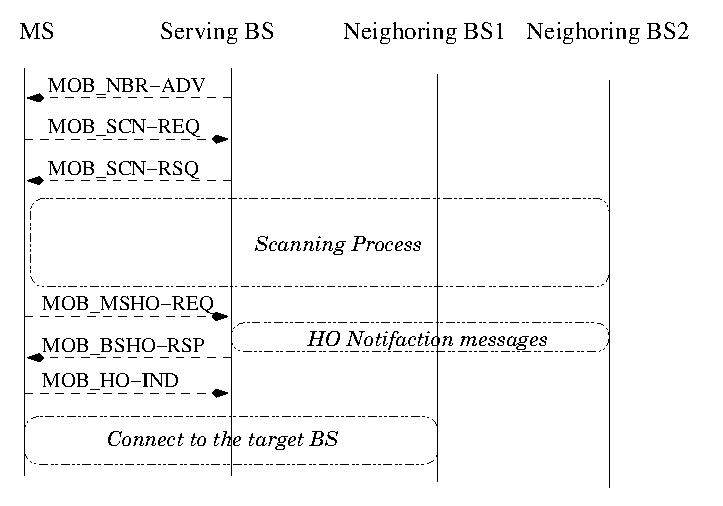
\includegraphics[]{iccs_handover}
\caption{切换流程示意图}
%\caption{Illustration of the handover procedure.}
\label{fig:chap_iccs_handover_algorithm_handover_flow}
\end{figure}
%%%%%%%%%%%%%%%%%%%%%%%%%%%%%%%%%%%%%%%%%%%%%%%%%%%%%%%%%%%%%%%%%%%

\subsection{切换成功概率与误比特率的关系分析}
不失一般性,我们假设在一次移动台的切换过程中有$M$($M \ge 2 $)个信令需要交换。设事件$A_i$表示一次信令的传送。 $p_i$是一次信令成功传送的概率,其中 $i = 0,1, \cdots, M-1 $。如果不考虑自动重传(ARQ)的策略,则有以下结论:

%%%%%%%%%%%%%%%%%%%%%%%%
\begin{equation}
\label{eq:chap_iccs_handover_algorithm_pro_mess_no_tran}
P(A_{i})=p_{i},\; P(\bar{A}_{i})=1- p_{i}, i=0,1,\cdots,M-1
\end{equation}
%%%%%%%%%%%%%%%%%%%%%%%%
在WiMAX切换过程中,重传策略不但可以用来对用户数据的传递,也通常用于保证信令消息的可靠传送。所以,根据切换信令的要求,这里我们假设一个信令消息如果不能被对方成功接收,将会被重传定时器激发再次重传过程,并且直到接到对方反馈为止。那么,考虑了重传策略后,则公式 (\ref{eq:chap_iccs_handover_algorithm_pro_mess_no_tran})可以重新写为下面的式子:

%%%%%%%%%%%%%%%%%%%%%%%%
\begin{equation}
\label{eq:chap_iccs_handover_algorithm_Pro_basic01}
P(A_{i})=\sum_{j=1}^{N_{i}}q_{i}^{j-1}p_{i}=\sum_{j=1}^{N_{i}}
(1-p_{i})^{j-1}p_{i},\quad N_{i}\geq1,
\end{equation}
%%%%%%%%%%%%%%%%%%%%%%%%
其中,$N_i$表示在一次切换过程中,第$i$个信令消息在成功接收到前会被传递的次数。在切换过程中有$M$个信令消息,那么,只有$M$个信令都收到,切换才认为是成功的,所以切换成功的概率可表示为:

%%%%%%%%%%%%%%%%%%%%%%%%%%
\begin{equation}
\label{eq:chap_iccs_handover_algorithm_Pro_basic02}
P_{succ}=\prod_{i=0}^{M-1}P(A_{i})=\prod_{i=0}^{M-1}
\left[\sum_{j=1}^{N_{i}}(1-p_{i})^{j-1}p_{i}\right].
\end{equation}
%%%%%%%%%%%%%%%%%%%%%%%%%%
在WiMAX的物理层中使用了交织信道编码的技术,所以这里的无线信道可以假设为无记忆的信道。那么,$p_i$将主要与移动台和基站之间的无线信道的误比特率有关。我们用数学公式表示如下:

%%%%%%%%%%%%%%%%%%%%%%%%%%
$$
p_{i}=\varphi(P_{b}(\gamma_{b}),\: L_{i}),
$$
%%%%%%%%%%%%%%%%%%%%%%%%%%
其中,$P_b(\gamma_b)$是当接收比特信噪比为$\gamma_b$的误比特概率。这样,如果设第$i$个信令消息的长度为$Li$,则有

%%%%%%%%%%%%%%%%%%%%%%%%
\begin{equation}\label{eq:chap_iccs_handover_algorithm_Pro_basic03}
p_{i}=[1-P_{b}(\gamma_{b})]^{L_{i}}.
\end{equation}
%%%%%%%%%%%%%%%%%%%%%%%%
所以,将公式(\ref{eq:chap_iccs_handover_algorithm_Pro_basic03})代入公式(\ref{eq:chap_iccs_handover_algorithm_Pro_basic02}),可以得到切换成功概率与无线信道识比特率之间的关系。

%%%%%%%%%%%%%%%%%%%%%%%%%
\begin{align}
\label{eq:chap_iccs_handover_algorithm_Pro_basic_final}
\notag P_{succ}&=\prod_{i=0}^{M-1}P(A_{i})\\
&=\prod_{i=0}^{M-1}\left\{ \sum_{j=1}^{N_{i}}\left\{ 1-[1-P_{b}(\gamma_{b})]^{L_{i}}\right\} ^{j-1} \cdot[1-P_{b}(\gamma_{b})]^{L_{i}}\right\}
\end{align}
%%%%%%%%%%%%%%%%%%%%%%%%%%

%%%%%%%%%%%%%%%%%%%%%%%%%%%%%%%%%%%%%%%%%%%%%%%%%%%%%%%%%%%%%%%%%%%%%
\begin{figure}[htbp]
\begin{centering}
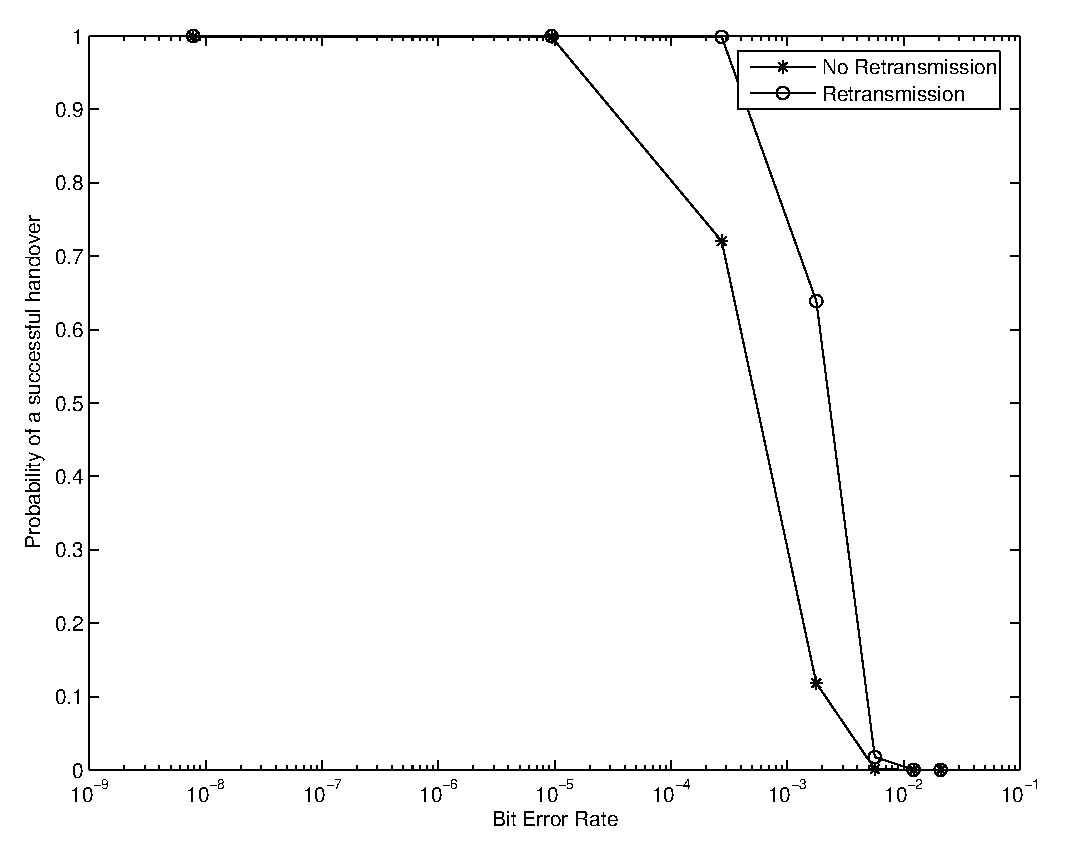
\includegraphics[scale=0.6]{iccs_ber_prob}
\par\end{centering}
%%\caption{Probability of a handover success as a function of BER, where $M=5,\sum_{i=0}^{M-1}N_i<=50,L_i=250$ bits in this case.}
\caption{切换成功概率与误比特率的关系。在此例中,$M=5,\sum_{i=0}^{M-1}N_i<=50,L_i=250$}
\label{fig:chap_iccs_handover_algorithm_PBER}
\end{figure}
%%%%%%%%%%%%%%%%%%%%%%%%%%%%%%%%%%%%%%%%%%%%%%%%%%%%%%%%%%%%%%%%%%%%%
这里,我们给出公式(\ref{eq:chap_iccs_handover_algorithm_Pro_basic_final})的一个例子,如图 \ref{fig:chap_iccs_handover_algorithm_PBER}。可以明显地看出,对于固定的$N_i$,切换的成功概率$P_{succ}$随着误比特概率$P_b(\gamma_b)$的增大而降低。当误比特率较大时(在$10^{-4}$到$10^{-2}$之间),使用重传策略会有效地改善切换的成功率。

\subsection{切换成功概率与移动台速度的关系}
上一节的分析指出了切换成功概率也两个重要的参数有关:一是信道的误比特率,二是信令消息的重传次数。在一个实际的WiMAX网络中,这二者都与移动台的移动速度有关。首先,移动的速度会影响多谱勒频率偏移,进而影响信道的误比特率,最终对信令消息的重传次数产生影响。同时,两个相邻基站覆盖的交叠部分是有限距离的,所以不能做到无限制的重传。所以,一个快速移动的终端要求基站切换的速度与时间也有更严格的要求。基于上述的考虑可知,通常情况下,移动台的移动速度越快,切换成功的概率会越低。
为了定量的分析起见,我们假设在切换过程中,对信令处理的时间是可以忽略不计的。所以,在整个切换过程中的延时可以写为下面的式子,

%%%%%%%%%%%%%%%%%%%%%%%%%%%%%%%%%%%%%
$$
T_{M}=(N_{0}+N_{1}+\cdots+N_{M-1})\cdot T_{retx}+M\cdot T_{prop},
$$
%%%%%%%%%%%%%%%%%%%%%%%%%%%%%%%%%%%%%
其中,$N_i$表示第$i$个信令传递的次数。$T_{retx}$是同一信令消息重传的计时器间隔,$T_{prop}$是在移动台与基站之间的承载信令的电磁波传播所需时间。

我们用$D_{overlap}$表示在移动台移动方向上两个相邻基站的覆盖范围的重叠部分的的距离。如图\ref{fig:chap_iccs_handover_bs}如示。$v_m$是移动台的移动速度。则有在一次成功的基站切换过程中,下面的约束需要满足:

%%%%%%%%%%%%%%%%%%%%%%%%%%%%%%%%
\begin{equation}
T_{M}<\frac{D_{overlap}}{v_{m}}.
\end{equation}
%%%%%%%%%%%%%%%%%%%%%%%%%%%%%%%
在这个约束下,一次成功切换的概率可以进一步被改写为下面的式子

%%%%%%%%%%%%%%%%%%%%%%%
\begin{equation}
P_{succ}=\left\{
\begin{array}{ll}
\prod_{i=0}^{M-1}\left[\sum_{j=1}^{N_{i}}(1-p_{i})^{j-1}p_{i}\right],
& \mbox{if }T_{M}<\frac{D_{overlap}}{v_{m}},\\
\\0, & \mbox{others},
\end{array}\right.\label{eq:chap_iccs_handover_algorithm_Pro_basic_final00}
\end{equation}
%%%%%%%%%%%%%%%%%%%%%%%
其中,

%%%%%%%%%%%%%%%%%%%%%%%%
$$
T_{M}=\sum_{i=0}^{M-1}(N_{i})\cdot T_{retx}+M\cdot T_{prop}
$$
%%%%%%%%%%%%%%%%%%%%%%%%

%%%%%%%%%%%%%%%%%%%%%%%%
$$
p_{i}=[1-P_{b}(\gamma_{b})]^{L_{i}}.
$$
%%%%%%%%%%%%%%%%%%%%%%%%
这里,我们使用Rayleigh信道。平均接收符号的信噪比(energy-to-noise)可以表示为:\cite{GLST:PMC2002}\cite{Leung:WCNC2005}
%%%%%%%%%%%%%%%%%%%%%%%%
\begin{equation}
\bar{\gamma}_{s}=\frac{1}{1-\frac{1}{N^{2}}\left[N+2\sum_{i=1}^{N-1}\left(N-i\right)J_{0}(2\pi f_{m}T_{s}i) \right]
+\frac{NT_{s}}{E_s/N_{0}}},
\end{equation}
%%%%%%%%%%%%%%%%%%%%%%%

$N$是OFDM子载波的个数,$T_s$是一个K阶QAM调制的符号在一个子载波上的传输时间。$N_0$是噪声功率, $E_s$是传送每个符号的平均能量。$f_{m}=fv_{m}/c $是最大的多谱勒频偏,$f$为载波频率,$v_m$为移动台的速度,$c$为光速。那么相应的接收到的平均比特信噪比为
%%%%%%%%%%%%%%%%%%%%%%%%
\begin{align}
\bar{\gamma}_{b}&= \frac{ \bar{\gamma}_s} {\log_2K} \\
&=\frac{1/\log_{2}K}{1-\frac{1}{N^{2}}\left[N+2\cdot \sum_{i=1}^{N-1}\left(N-i\right) J_{0}(2\pi f_{m}T_{s}i) \right]
+\frac{NT_{s}}{\log_{2}K}\left(\frac{1}{E_{b}/N_{0}}\right)}
\end{align}
其中,
\begin{equation*}
J_{0}(2\pi f_{m}T_{s}i) = \frac{1}{\pi}\int_0^\pi \cos(2\pi f_m T_{s}i \sin \theta) d \theta
\end{equation*}
%%%%%%%%%%%%%%%%%%%%%%%
此处,我们假设以Clarke-Jakes的模型为基础的Rayleigh信道模型。

%其中,$Y$定义为
%%%%%%%%%%%%%%%%%%%%%%%%
%$$
%Y=\sum_{i=1}^{N-1}\left(N-i\right)J_{0}(2\pi f_{m}T_{s}i)
%$$
%%%%%%%%%%%%%%%%%%%%%%%%%
对于M阶的QAM调试(如果$M=4$,调制的方式是QPSK;如果$M=16$,那么就是16-QAM)。
我们假设在接收端可以进行出错的符号检测。那么对于当接收比特能量与噪声比为$\gamma_b$时,误比特概率(bit error, BER)为$P_b(\gamma_b)$可以写为:

%%%%%%%%%%%%%%%%%%%%%%%
\[
{{P}_{b}}=\int\limits_{0}^{\infty }{{{P}_{b}}(\gamma ){{f}_{{{\gamma }_{b}}}}(}\gamma )d\gamma
\]
%%%%%%%%%%%%%%%%%%%%%%%%
其中,$f_{\gamma_b}$是Rayleigh信道模型的比特能量与噪声比的概率密度函数。它定义如下:

%%%%%%%%%%%%%%%%%%%%%%%%%
\[{{f}_{{{\gamma }_{b}}}}(\gamma )=\frac{\exp (\frac{-\gamma }{{{{\bar{\gamma }}}_{b}}})}{{{{\bar{\gamma }}}_{b}}},\gamma \ge 0\]
%%%%%%%%%%%%%%%%%%%%%%%%%%%%
我们假设载波间的干扰(ICI)为高斯白噪声。根据文献\cite{Leung:WCNC2005},这个近似在$1024\ge N \ge 256$是比较精确的。那么,对于M阶的QAM和Gray码,可以有如下的近似,

%%%%%%%%%%%%%%%%%%%%%%%
\begin{equation}
P_b(\gamma_b) \approx \frac{P_M(\gamma_s)}{\log_2 M}
\end{equation}
%%%%%%%%%%%%%%%%%%%%%%%
其中,$P_M$是符号的错误概率。特别对于QPSK,有

%%%%%%%%%%%%%%%%%%%%%%%%
\begin{align}
\label{eq:chap_iccs_handover_algorithm_BER_V}
P_{b}(\gamma_{b})&= Q\left(\sqrt{2\gamma_{b}}\right).\\
Q(x) &= \int^x_{-\infty} \frac{1}{\sqrt{2\pi}}e^{-y^2/2}dy
\end{align}
%%%%%%%%%%%%%%%%%%%%%%%%
把公式(\ref{eq:chap_iccs_handover_algorithm_Pro_basic_final00})和公式( \ref{eq:chap_iccs_handover_algorithm_BER_V})合并则有下面的结果。我们可以得到以移动台速度为变量的一个切换成功概率函数。如图\ref{fig:chap_iccs_handover_algorithm_Pro_V}

%%%%%%%%%%%%%%%%%%%%%%%%%%%%%%%%%%%%%%%%%%%%%%%%%%%%%%%%%%%%%%%%%%%%
\begin{figure}[htbp]
\begin{centering}
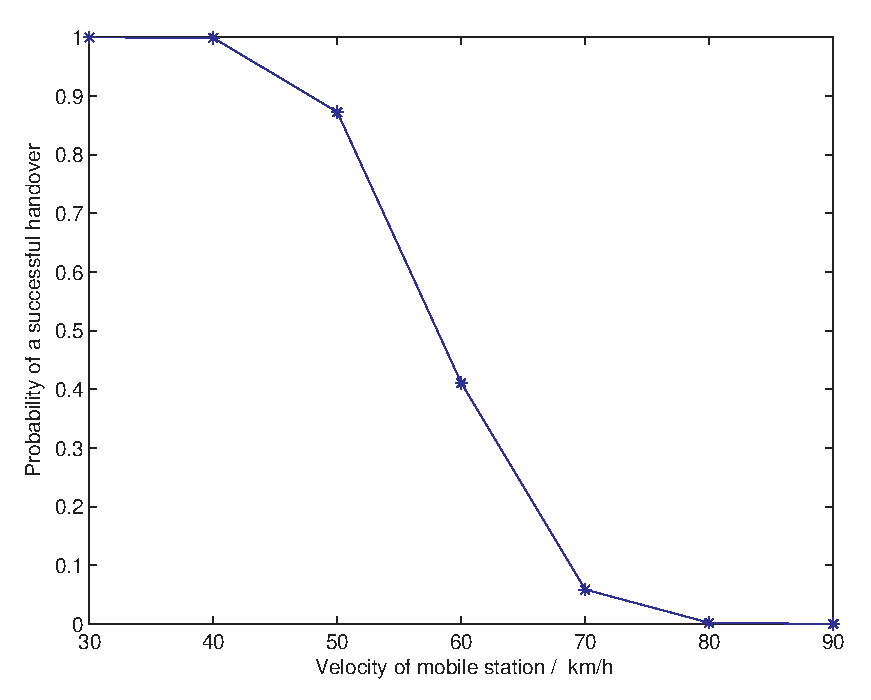
\includegraphics[scale=0.7]{iccs_speed_prob_theroy}
%%\caption{The probability of a handover success as a function of MS's velocity, where $M=5, \sum_{i=0}^{M-1}N_i=50, L_i=250$ bits in this case.}
\caption{切换成功概率与用户的移动速度关系,在本例中$M=5, \sum_{i=0}^{M-1}N_i=50, L_i=250$}
\label{fig:chap_iccs_handover_algorithm_Pro_V}
\end{centering}
\end{figure}
%%%%%%%%%%%%%%%%%%%%%%%%%%%%%%%%%%%%%%%%%%%%%%%%%%%%%%%%%%%%%%%%%%%%

很明显,随着移动的速度增快,切换成功概率会显著下降。这样会极大地影响了切换的过程。所以说,如果在高速移动状态下,切换对于移动台来说需要额外的处理。

\section{高速移动下的切换方案}
在高速移动状态下,为了提高移动台的切换成功概率,除了可以增加重传的次数以外,我们也需要建立更加可靠的通信链路的传输机制来传送信令消息。本节我们讨论了前向纠错编码的特点,并采用此技术来改善传输的误码率。前向纠错编码是通过发送端使用冗余比特数来提供差错保护。这些额外的冗余比特可以帮助接收端检测并纠正错误。如果采用了前向纠错的技术,数据重传的次数也会降低。根据WiMAX的标准,切换信令的消息大小约为50到80个字节左右。同时由于所要无线信道的限制及交换的信令消息较多,所以要在满足要求的基础上尽可能减少冗余比特数。
不同的前向纠错编码方案可以提供不同的纠错能力。对于同一种前向纠错码而言,冗余比特数越多,纠错能力也超强。所以下面我们要定量的讨论冗余比特的个数。对于一个给定的移动台速度,我们要能基于所要达到的切换成功率来计算出冗余比特数。为了简单起见,我们假设切换消息信令的长度不变,设切换消息传输一次的成功的概率为$\tilde{p}$以替换公式(\ref{eq:chap_iccs_handover_algorithm_Pro_basic_final00})中的$p_i$,如下

%%%%%%%%%%%%%%%%%%%%%%%%%%%%%%%%%%%
\begin{align}
\notag P_{succ} &= \prod_{i=0}^{M-1}P(A_{i})\\
&= \prod_{i=0}^{M-1}\left[\sum_{j=1}^{N_{i}}(1-p_{i})^{j-1}p_{i}\right]\\
\notag &\thickapprox\sum_{i=M}^{S}{i-1 \choose M-1}\cdot\widetilde{p}^{M}(1-\widetilde{p})^{i-M}
\end{align}
%%%%%%%%%%%%%%%%%%%%%%%%%%%%%%%%%%

其中,$S=\sum_{i=0}^{M-1}N_{i}$是总共重传的次数。根据\ref{section_iccs_handover_algorithm_mobility_analysis}节的分析,可以得到如下的公式:

%%%%%%%%%%%%%%%%%%%%%%%%%%%%%%%%%%
\begin{align*}
S & = \sum_{i=0}^{M-1}N_{i}\\
  & = \left\lfloor \frac{(\frac{D_{overlap}}{v_{m}}-MT_{prop})}
        {T_{retx}}\right\rfloor \leq\frac{(\frac{D_{overlap}}{v_{m}}
        -MT_{prop})}{T_{retx}}.
\end{align*}
%%%%%%%%%%%%%%%%%%%%%%%%%%%%%%%%%%

这样,我们就可根据相邻基站覆盖交叠的距离$D_{overlap}$和移动台的速度$v_m$,得到参数$S$;并根据所要求的$P_{succ}$进一步计算得每一个信令的成功传输的概率值。如果使用Reed-Solomon(R-S)纠错编码,我们可以推导出如下的式子。

%%%%%%%%%%%%%%%%%%%%%%%%%%%%%
\begin{equation}\label{eq:chap_iccs_handover_algorithm_FEC_Pro_final}
\tilde{p}\approx\frac{2^{k-1}}{k(2^{k}-1)^{2}}\sum_{j=t+1}^{2^{k}-1}j
\cdot{2^{k}-1\choose j}_{}^{}\cdot p^{j}(1-p)^{2^{k}-1-j},
\end{equation}
%%%%%%%%%%%%%%%%%%%%%%%%%%%%%
其中, $t=\lfloor\frac{N-k}{2}\rfloor$ 是编码的符号纠错能力,$N$是全部的比特数,$k$是信令消息的比特数, $\lfloor{x}\rfloor$表示不超过$x$的最大整数。那么冗余比特数$N-k$可以确定下来。图 \ref{fig:chap_iccs_handover_algorithm_AFEC_bits} 表明了在想要达到不同的切换成功概率($50\%,80\%,99\%$)下,在不同的速度下,移动台所需的冗余比特数。

%%%%%%%%%%%%%%%%%%%%%%%%%%%%%%%%%%%%%%%%%%%%%%%%%%%%%%%%%%%%%%%%%%%%%%%%%%%
\begin{figure}[htbp]
\begin{centering}
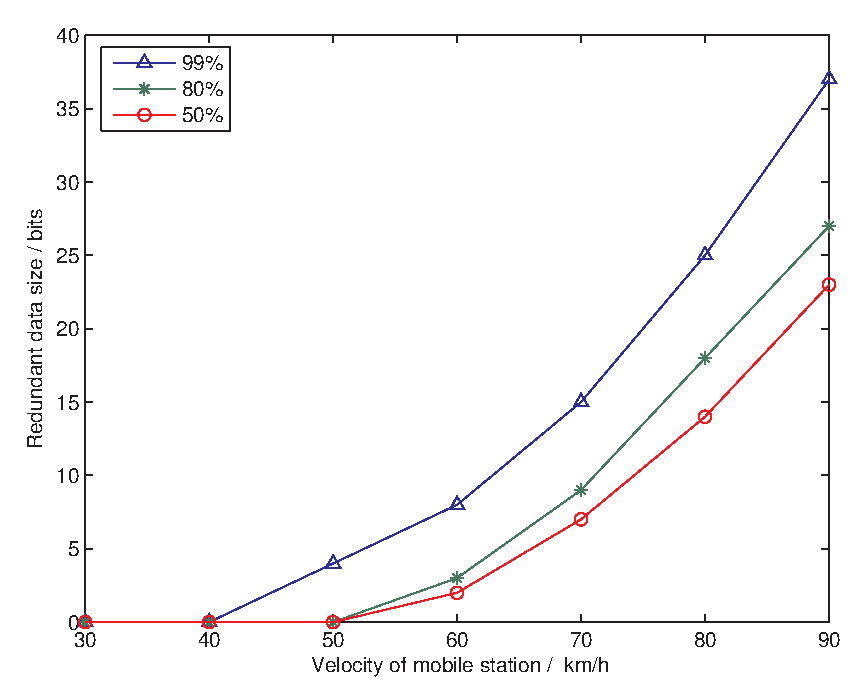
\includegraphics[scale=0.7]{iccs_speed_size_theory}
\caption{RS码中的冗余比特数与移动台速度之间的关系,其中,假设$k=250$比特}
\label{fig:chap_iccs_handover_algorithm_AFEC_bits}
\end{centering}
\end{figure}
%%%%%%%%%%%%%%%%%%%%%%%%%%%%%%%%%%%%%%%%%%%%%%%%%%%%%%%%%%%%%%%%%%%%%%%%%%%

如图 \ref{fig:chap_iccs_handover_algorithm_AFEC_bits}所示,当移动台的速度越快,那么为了达到所要设定的切换成功概率,所需的冗余比特数也越多。例如,为了能够达到$80\%$的成功概率,如果移动台的速度分别是50,70, 90 km/h,那么所需的冗余比特数是2,10,28。通过上面的分析,我们可以使用一种自适应的方法根据不同的移动台速度来增加所需的冗余比特。

\section{仿真实验与结果}
我们通过计算机仿真实验来验证和评估我们的自适应前向纠错方案。在实验中,我们使用了NS-2仿真模拟器和修改了的NIST的WiMAX仿真代码。实验主要的实验设置参数如表格\ref{chap_iccs_table_I} 所示。

%%%%%%%%%%%%%%%%%%%%%%%%%%%%%%%%%%%%%%%%%%%%%%%%%%%%%%%%%%%%%%%%%%%%%
\begin{table}[h]
\centering
%\begin{centering}
\caption{仿真实验的主要参数配置}\label{chap_iccs_table_I}
\begin{tabular*}{0.99\textwidth}{p{7cm} p{7cm}} 
\toprule 
Parameters  &  Values \\
\midrule
Overlap distance  & 200 meters\tabularnewline 
Bandwidth  & 5 MHz\tabularnewline 
Carrier Frequency  & 2.5 GHz\tabularnewline 
FFT size  & 512\tabularnewline
Channel mode  & Rayleigh channel\tabularnewline 
FEC code  & Reed-Solomon code\tabularnewline 
Velocity  & 30-90 km/h\\
\bottomrule
\end{tabular*}
%\end{centering}
\end{table}
%%%%%%%%%%%%%%%%%%%%%%%%%%%%%%%%%%%%%%%%%%%%%%%%%%%%%%%%%%%%%%%%%%%%%

这里,我们采用的是自适应的前向纠错码方案。如图 \ref{fig:chap_iccs_results}所示的仿真结果是在认定理论计算得到的,在切换成功概率为50\%,80\%,99\%的情况下所需要的冗余比特数。最终得到的仿真所得的实验结果。对于每一组实验参数,仿真进行1000次,然后取结果的平均值来得到可靠的统计结果。从图中我们可以看到,在移动台的速度较低时,增加一些冗余比特会使得切换成功的概率会显著增加到接近于~1。而当速度逐渐增大后,对于目标为50\%的曲线,切换成功率会下降,但仍然会保持在50\%以上。这说明,在保证高切换成功率,如99\%,所增加的冗余比特数较多,我们的方案略显些保守。而且我们也注意到,在速度为70km/h时,理论成功率50\%的曲线存在一个极值点。经过分析,我们认为有两个原因会造成一是,对于我们使用的Rayleigh信道模型所计算得到的前向纠错的冗余比特不是十分准确,二是在冗余比特数与移动台速度之间并不是一个线性的关系。我们使用了最大的冗余比特数来满足前向纠错码的要求。

%%%%%%%%%%%%%%%%%%%%%%%%%%%%%%%%%%%%%%%%%%%%%%%%%%%%%%%%%%%%%%%%%%%%%
\begin{figure}[htbp]
\begin{centering}
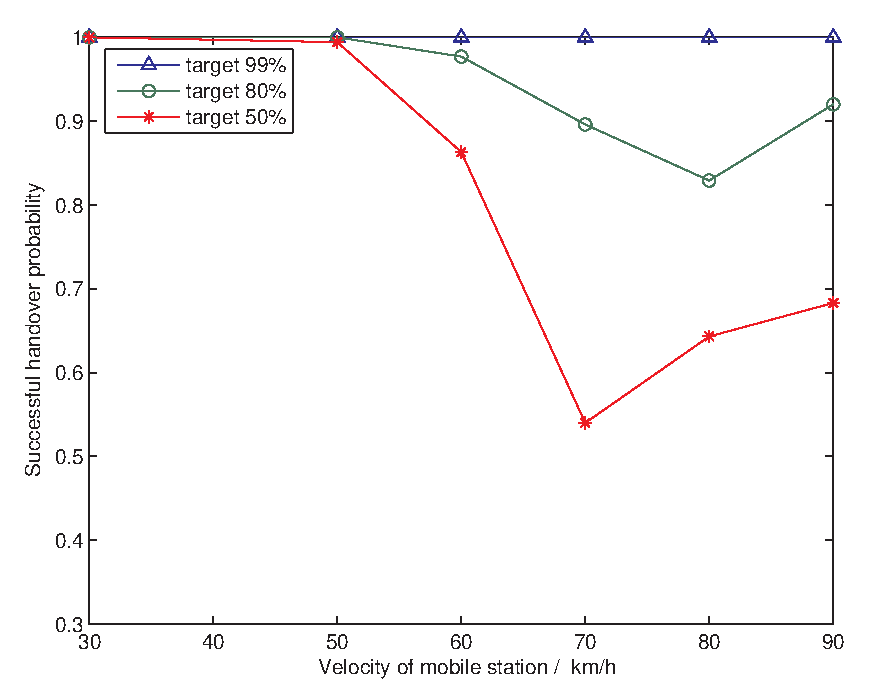
\includegraphics[scale=0.8]{iccs_speed_prob_simu}
%\caption{Simulation results of the probability of a handover success using the proposed adaptive FEC scheme.}
\caption{仿真实验的结果}
\label{fig:chap_iccs_results}
\end{centering}
\end{figure}
%%%%%%%%%%%%%%%%%%%%%%%%%%%%%%%%%%%%%%%%%%%%%%%%%%%%%%%%%%%%%%%%%%%%%

\section{小结}
在本章中,我们以WiMAX网络为例分析了移动台的移动速度对切换成功率的影响。分析的结果表明,由于移动台的速度增加会导致无线传输的信道变差,进而使得切换信令不能正常收发。又由于切换操作是时间受限的,所以在设计切换时要两方面同时考虑。根据理论分析,我们提出了一个简单有效的自适应前向纠错方案,通过理论计算就可以提到在不同速度下所需的冗余比特数,可以满足在不同移动速度下的切换设计需要。最后仿真实验验证了我们的理论分析和所提出前向纠错方案的正确性。
%chapter_end
